\vspace{-.05in}
\section{Proposed Approach}
Given a trained DNN classifier $\bff$, a paired OOD detector $\calD_\gamma$, and a set of concepts $\bfC$, we address the following questions: \textbf{1)} \emph{Are the concepts sufficient to capture the prediction behavior of both the classifier and OOD detector?} (see \S~\ref{sec:completeness_score}); \textbf{2)} \emph{Do the concepts show clear distinctions in their scores between detected-ID data and detected-OOD data?} (see \S~\ref{sec:separability_score}). 
We first propose new metrics for quantifying the set of learned concepts, followed by a general framework for learning concepts that possess these properties (see \S~\ref{sec:concept_learning}).
% We propose a general framework for learning a set of concepts that possess these properties (\S~\ref{sec:concept_learning}).
% This section explains our evaluation metrics and methods: (1) how to gauge the utility of a given set of concepts for OOD detector explanation, and (2) a general learning algorithm to discover concepts that \jihye{incomplete yet}

\subsection{Metric for Detection Completeness}
\label{sec:completeness_score}
% To address the question of whether a set of learned concepts are sufficient to capture the behavior of the classifier and OOD detector, we next define completeness scores with respect to the classification task and the detection task. 
%
% We address the following questions: 1) \textit{are the set of concepts sufficient to similarly match the behavior of the original classifier $\bff$}, and 2) \textit{are the set of concepts sufficient to similarly match the behavior of the OOD detector $\calD_\gamma$?} 
% Such properties would indicate that the concepts are appropriate for describing the behavior of $\bfC$ and $\calD_\gamma$.
%
% Given a trained DNN classifier $\bff$ and a trained OOD detector $\calD_\gamma$, our goal is to learn a set of concepts that can provide explanations for the predictions of the classifier and detector.
% To this end, we first propose new metrics for quantifying a set of learned concepts, followed by a general framework for learning a set of concepts.
% Given a sufficient set of concepts $\bfC$, the classifier in the concept world should be able to closely approximate the prediction performance of the original classifier.
% Likewise, the detector in the concept world should be able to closely approximate the detection performance of the original detector.
% In order to concretely quantify these properties, we hereby define a 
% completeness score for the set of concepts with respect to the classification task and the OOD detection task.
%
\begin{definition}
\label{def:completeness_class}
Given a trained DNN classifier $\bff = \bfh \circ \bfphi\,$ and a set of concept vectors $\bfC$, the {\em classification completeness} with respect to $\Pin(\bfx, y)$ is defined as \citep{yeh2020completeness}:
\begin{align*}
% \label{equ: completeness-classification}
    &\eta^{}_\bff(\bfC) := \\
    &\frac{\textrm{sup}_\bfg \,\expec_{(\bfx, y) \sim \Pin} \!\big[ \indicator[ y = \argmax_{y'} h_{y'}(\recphi(\bfx)) ] \big] ~-~ a_r}{\expec_{(\bfx, y) \sim \Pin} \!\big[ \indicator[y = \argmax_{y'} h_{y'}(\bfphi(\bfx))] \big] ~-~ a_r}
\end{align*}
where $a_r = 1 / L$ is the accuracy of a random classifier.
\end{definition}
The denominator of $\eta^{}_\bff(\bfC)$ is the accuracy of the original classifier $\bff$, while the numerator is the maximum accuracy that can be achieved by the concept-world classifier.
% while the numerator is the maximum accuracy that can be achieved in the concept world using the feature representation reconstructed from the concept scores.
The maximization is over the parameters of the neural network $\bfg$ that reconstructs the feature representation from the vector of concept scores.
%\textcolor{blue}{We parameterize $\bfg$ using a neural network, and the maximization in the numerator is over the parameters of $\bfg$.}
% \textcolor{blue}{The expectation is estimated using a held-out test dataset $\Dinte$ from the ID distribution.}

\begin{definition}
\label{def:completeness_detec}
Given a trained DNN classifier $\bff = \bfh \circ \bfphi$, a trained OOD detector with score function $S(\bfx, \bff)$, and a set of concept vectors $\bfC$, we define the {\em detection completeness score} with respect to the ID distribution $\Pin(\bfx, y)$ and OOD distribution $\Pout(\bfx)$ as follows:
%\vspace{-2mm}
\begin{align}
\label{equ: completeness-detection}
    \eta^{}_{\bff, S}(\bfC) 
    ~:=~ \frac{\textrm{sup}_\bfg \,\textrm{AUC}(\bfh \circ \recphi) ~-~ b_r}{\textrm{AUC}(\bfh \circ \bfphi) ~-~ b_r},
\end{align}
% where $\recphi(\bfx) = \bfg(\bfv_{\bfC}(\bfx))$ is the feature representation reconstructed from the concept scores, 
where $\textrm{AUC}(\bff)$ is the area under the ROC curve of an OOD detector based on $\bff$, defined as $\,\textrm{AUC}(\bff) \,:=\, \expec_{(\bfx, y) \sim \Pin} \expec_{\,\bfx^\prime \sim \Pout} \indicator\big[ S(\bfx, \bff) \,>\, S(\bfx^\prime, \bff) \big]$,
%
% \begin{align}
% \label{equ:auroc_ideal}
% \textrm{AUC}(\bff) ~:= \!\!\expec_{(\bfx, y) \sim \Pin} \expec_{\,\bfx^\prime \sim \Pout} \indicator\big[ S(\bfx, \bff) \,>\, S(\bfx^\prime, \bff) \big],
% \end{align}
%
and $b_r = 0.5$ is the AUROC of a random detector.
\end{definition}
% As with the classification completeness, the maximization in the numerator is over the parameters of the fully-connected network $\bfg$ that reconstructs the feature representation from the vector of concept scores \jihye{is this sentence necessary?}.

The numerator is the maximum achievable AUROC in the concept world using the reconstructed representation from concept scores.
In practice, $\textrm{AUC}(\bff)$ is estimated using the test datasets $\Dinte$ and $\Doutte$.
%
% \begin{align*}
%     \widehat{\textrm{AUC}}(\bff) \,=\, \frac{1}{|\Dinte|\,|\Doutte|} \!\!\mysum_{(\bfx, y) \in \Dinte} \mysum_{~\bfx^\prime \in \Doutte} \!\!\!\indicator\big[ S(\bfx, \bff) > S(\bfx^\prime, \bff) \big]. 
% \end{align*}
%
Both the classification completeness and detection completeness are designed to be in the range $[0, 1]$. However, this is not strictly guaranteed since the classifier or OOD detector in the concept world may empirically have a better (corresponding) metric on a given ID/OOD dataset.
Completeness scores close to $1$ indicate that the set of concepts $\bfC$ are close to complete in characterizing the behavior of the classifier and/or OOD detector.

%\vspace{-0.1in}
\subsection{Concept Separability Score}
\label{sec:separability_score}
\mypara{Concept Scores.}
% We start by formalizing how to compute a representative score for concepts given an input, which will be used for evaluation in Section \ref{sec:completeness_score} and \ref{sec:separability_score}.
In Section \ref{sec:concept_projection}, we introduced a projection matrix $\bfC \in \reals^{d_\ell \times m}$ that maps $\bfphi(\bfx)$ to $\bfv_{\bfC}(\bfx)$, and consists of $m$ unit concept vectors $\,\bfC = [\bfc_1 \cdots \bfc_m]$. 
The inner product between the feature representation and a concept vector is referred to as the {\em concept score}, and it quantifies how close an input is to the given concept~\citep{kim2018tcav, ghorbani2019ace}.
% \ap{Does this need a cite? or is this our term?}
%
Specifically, the concept score corresponding to concept $i$ is defined as $\,\bfv_{\bfc_i}(\bfx) := \langle \bfphi(\bfx), \bfc_i \rangle = \bfphi(\bfx) \,\bfc_i \in \reals^{a_\ell b_\ell}$. 
%
% the $a_\ell \times b_\ell$ times concatenation over the standard inner-products (between vectors) $\,\langle \bfphi^{p,q}(\bfx), \bfc_i \rangle \in \reals, ~\forall p, q \in [a_\ell] \times [b_\ell]$, where $\bfphi^{p,q}$ is the feature representation corresponding to the $(p, q)$-th patch of input $\bfx$ (\ie receptive field).
% That is, $\bfv_{\bfc_i}^{(p,q)}(\bfx)$ is the concept score of $(p, q)$-th patch of $\bfx$ with respect to $i$-th concept, and if it is a large positive (or negative) value, then the corresponding part of input is positively (or negatively) aligned with the concept.
%
The matrix of concept scores from all the concepts is simply the concatenation of the individual concept scores, \ie $\VC(\bfx) = \bfphi(\bfx) \,\bfC = [\bfv_{\bfc_1}(\bfx) \cdots \bfv_{\bfc_m}(\bfx)] \in \reals^{a_\ell b_\ell \times m}$.
% When $p = q = 1$ for fully-connected layers (\ie the receptive field of $\bfphi$ corresponds to the entire input $\bfx_i$), $\langle \bfphi(\bfx_i),~\bfc_j \rangle$ is a scalar concept score that represents the input.
% On the other hand, when $p, q > 1$, to obtain a scalar concept score for a given input, we take the maximum absolute concept score across the $p \times q$ patches, corresponding to $p \times q$ feature representations.
% To define the overall closeness of an input $\bfx_i$ and the concept $\bfc_j$ with a scalar concept score, we take the maximum absolute concept score across the $p \times q$ patches of $\bfx_i$.
%
% \ap{Are p and q referring to the patch position? If so, why are (1,1), (1, -), and (-, 1) excluded by p, q > 1?}
%
% When $p, q > 1$ (unless a fully-connected layer is of interest), where the receptive field of $\bfphi$ corresponds to the entire input $\bfx_i$), 
%
We also define a dimension-reduced version of the concept scores that takes the maximum of the inner-product over each $a_\ell \times b_\ell$ patch as follows: $\TVC(\bfx)^T = [\widetilde{v}_{\bfc_1}(\bfx), \cdots, \widetilde{v}_{\bfc_m}(\bfx)] \in \reals^m$, where $\,\widetilde{v}_{\bfc_i}(\bfx) = \max_{p, q} |\langle \bfphi^{p,q}(\bfx), \bfc_i \rangle| \in \reals$. Here $\bfphi^{p,q}(\bfx)$ is the feature representation corresponding to the $(p, q)$-th patch of input $\bfx$ (\ie receptive field~\citep{araujo2019computing}).
This reduction operation is done to capture the most important correlations from each patch, and the $m$-dimensional concept score will be used to define our concept separability metric as follows.
%
% We next discuss the evaluation criteria of concepts for explaining an OOD detector, followed by a general learning algorithm to discover concepts that satisfy these criteria.

\iffalse

% The intuition behind taking a maximum score across the patches of input is as follows.
Suppose $\bfc_j$ represents a striped pattern and $\bfx_i$ is an image of a zebra standing on grass.
The patch of greenery background should get a low concept score, while a patch of the zebra's body should get high concept score.
% As the defining score for the stripe concept, we decide to take the score from the patch of zebra's body, out of all patches constituting the entire input image.
Out of all the patches constituting the input image, we take the maximum score (likely) corresponding to a patch of the zebra's body as the defining score for the striped concept.

% \somesh{Assumptions: enforcing separability of each individual separability --> anyway leads to better separability with combined concepts}
% \somesh{First describe the problem -what we want to do. There are these possible methods..... We chose this because of what. It should never appear like magic.}
% \somesh{Some curve -- accuracy vs separability something like that}

\jihye{need for/intuition behind separablility. Full elaboration on the idea behind separability in concept space -- fig \ref{fig:detection-separability}.} Other than the completeness scores of Eq. (\ref{equ: completeness-classification}) and Eq. (\ref{equ: completeness-detection}), we also want the concept scores between ID and OOD data to be easily distinguishable. This notion is captured by the \textit{separability} metric in Eq. (\ref{equ: distinguishability}). 

An important property that we would like to impose on the set of learned concepts for the OOD detection task is that the ID data and OOD data be well separated in the dimension-reduced concept-score space.
The motivation behind this requirement is two-fold.
The first is that we would like the concept scores to be highly distinguishable between the ID and OOD data (\eg Fig.~\ref{fig:detection-separability}), in order to effectively interpret the detector's decisions.
The second is that we would like the detector in the concept world Eq. (\ref{equ:detector_concept}) to have performance close to that of the original detector, which requires that the distribution of detector scores $\Scon(\cdot)$ from ID and OOD data be well separated.
% maybe we should say requirement of high detection completeness here?
This in-turn translates to a requirement of good separability (between ID and OOD) in the projected concept-score space.

\fi

% To ensure better interpretability of the concept-based explanations for OOD detection, 
We would like the set of concept-score vectors from the detected-ID class $\,V_{\textrm{in}}(\bfC) := \{\TVC(\bfx), ~\bfx \in \Dintr \cup \Douttr ~:~ \calD_\gamma(\bfx, \bff) = 1\}$, and the set of concept-score vectors from the detected-OOD class $\,V_{\textrm{out}}(\bfC) := \{\TVC(\bfx), ~\bfx \in \Dintr \cup \Douttr ~:~ \calD_\gamma(\bfx, \bff) = 0\}\,$ to be well separated.
Let $\,J_{\textrm{sep}}(V_{\textrm{in}}(\bfC), V_{\textrm{out}}(\bfC)) \in \reals$ define a general {\it measure of separability} between the two subsets, such that a larger value corresponds to higher separability. We discuss a specific choice for $J_{\textrm{sep}}$ for which it is possible to tractably optimize concept separability as part of the learning objective in Section \ref{sec:concept_learning}.

% $\,V_{\textrm{in}}(\bfC) := \{\TVC(\bfx) \in \reals^m, ~\bfx \in \Dintr \cup \Douttr ~:~ \calD_\gamma(\bfx, \bff) = 1\}$
% \ap{Should the following para be cut or shortened, given the space issue? I think we can retain the first sentence, but drop the rest and then continue on the Fisher's LDA sentence. Update: I went ahead and made the cuts. Undo if needed.}

\mypara{Global Concept Separability.} Class separability metrics have been well studied in the pattern recognition literature, particularly for the two-class case~\citep{fukunaga1990separ}\,\footnote{In our problem, the two classes correspond to ``detected-ID'' and ``detected-OOD''.}. 
%Distributional divergences such as the Kullback-Leibler and Hellinger distance can be used when the probability distribution of the two classes are known, and the divergence is tractable to compute.
%Non-parametric measures of class separability (\eg based on $k$-nearest neighbors) are also candidates here, but they are usually hard to optimize using gradient-based methods.
%In order to obtain a closed-form expression for the class separability, it is common to make simplifying assumptions on the class-conditional density (\eg multivariate Gaussian per class).
% We next propose a binary class separability 
%
%\mypara{Global Concept Separability.}
Motivated by Fisher's linear discriminant analysis (LDA), we explore the use of class-separability measures based on the within-class and between-class scatter matrices~\citep{murphy2012separ}.
The goal of LDA is to find a projection vector (direction) such that data from the two classes are maximally separated and form compact clusters upon projection. 
Rather than finding an optimal projection direction, we are more interested in ensuring that the concept-score vectors from the detected-ID and detected-OOD data have high separability.
% Given the set of concept-score vectors from the ID data $V_{\textrm{in}}(\bfC)$ and OOD data $V_{\textrm{out}}(\bfC)$, consider their within-class and between-class scatter matrices defined as
Consider the within-class and between-class scatter matrices based on $V_{\textrm{in}}(\bfC)$ and $V_{\textrm{out}}(\bfC)$, given by
\begin{align}
\label{eq:scatter_matrices}
\bfS_w ~&= \mysum_{\bfv \in V_{\textrm{in}}(\bfC)} (\bfv \,-\, \bfmu_{\textrm{in}})\,(\bfv \,-\, \bfmu_{\textrm{in}})^T \nonumber \\
&\,+\, \mysum_{\bfv \in V_{\textrm{out}}(\bfC)} (\bfv \,-\, \bfmu_{\textrm{out}})\,(\bfv \,-\, \bfmu_{\textrm{out}})^T, \\
%
\bfS_b ~&=~ (\bfmu_{\textrm{out}} \,-\, \bfmu_{\textrm{in}})\,(\bfmu_{\textrm{out}} \,-\, \bfmu_{\textrm{in}})^T,
\end{align}
where $\bfmu_{\textrm{in}}$ and $\bfmu_{\textrm{out}}$ are the mean concept-score vectors from $V_{\textrm{in}}(\bfC)$ and $V_{\textrm{out}}(\bfC)$ respectively.
We define the following separability metric based on the generalized eigenvalue equation solved by Fisher's LDA~\citep{fukunaga1990separ}: $J_{\textrm{sep}}(\bfC) ~:=~ J_{\textrm{sep}}(V_{\textrm{in}}(\bfC), V_{\textrm{out}}(\bfC)) ~=~ \textrm{tr}\big[\bfS_w^{-1} \,\bfS_b\big]$.
%
\iffalse

\begin{align}
\label{eq:separability_trace}
&J_{\textrm{sep}}(\bfC) ~:=~ J_{\textrm{sep}}(V_{\textrm{in}}(\bfC), V_{\textrm{out}}(\bfC)) ~=~ \textrm{tr}\big[\bfS_w^{-1} \,\bfS_b\big].
%
% &=~ \textrm{tr}\big[\bfS_w^{-1} \,(\bfmu_{\textrm{out}} \,-\, \bfmu_{\textrm{in}})\,(\bfmu_{\textrm{out}} \,-\, \bfmu_{\textrm{in}})^T\big] \nonumber \\
%
% &=~ (\bfmu_{\textrm{out}} \,-\, \bfmu_{\textrm{in}})^T \,\bfS_w^{-1} \,(\bfmu_{\textrm{out}} \,-\, \bfmu_{\textrm{in}}).
\end{align}

\fi
%
Maximizing the above metric is equivalent to maximizing the sum of eigenvalues of the matrix $\,\bfS_w^{-1} \,\bfS_b$, which in-turn ensures a large between-class separability and a small within-class separability for the detected-ID and detected-OOD concept scores.
We refer to this as a {\em global concept separability} metric because it does not analyze the separability on a per-class level.
% ~\footnote{See Appendix \ref{sec:appendix-perclass-completeness} and \ref{sec:appendix-perclass-separability} for the per-class variations of detection completeness and concept separability.}.
% it analyzes the ID and OOD data from all the $L$ classes.
The separability metric is closely related to the Bhattacharya distance, which is an upper bound on the Bayes error rate (see Appendix \ref{sec:appendix-BC-distance}).
% The discussion of comparing the global concept separability metric to Bhattacharya distance is in Appendix \ref{sec:appendix-BC-distance}.
We define the per-class variations of detection completeness and concept separability in a similar way in Appendix \ref{sec:appendix-perclass-completeness} and \ref{sec:appendix-perclass-separability}. 

% We use the shorthand notations $J_{\textrm{sep}}(\bfC)$ instead of $J_{\textrm{sep}}(V_{\textrm{in}}(\bfC), V_{\textrm{out}}(\bfC))$, and $J^y_{\textrm{sep}}(\bfC)$ instead of $J_{\textrm{sep}}(V^{y}_{\textrm{in}}(\bfC), V^{y}_{\textrm{out}}(\bfC))$ for brevity.

\iffalse
Besides a global concept-separability measure, it can also be informative to see if we can separate out concept scores for detected-OOD inputs classified as a certain class $c$, versus detected-ID inputs classified as $c$.
To obtain per-class concept separability, one can simply compute Eqn. \ref{eq:separability_trace} only with a subset of ID and OOD data whose predictions are class $y \in [L]$. 
We refer to this variation of Eqn. \ref{eq:separability_trace} as \textit{per-class concept separability}, denoted as $J_{\textrm{sep}}(V^{y}_{\textrm{in}}(\bfC), V^{y}_{\textrm{out}}(\bfC))$ (see Appendix \ref{sec:appendix-perclass-separability} for detailed description).
We sometimes use the shorthand notations $J_{\textrm{sep}}(\bfC)$ instead of $J_{\textrm{sep}}(V_{\textrm{in}}(\bfC), V_{\textrm{out}}(\bfC))$, and $J^y_{\textrm{sep}}(\bfC)$ instead of $J_{\textrm{sep}}(V^{y}_{\textrm{in}}(\bfC), V^{y}_{\textrm{out}}(\bfC))$ for brevity.
\fi

\iffalse

% Separability literature (BC distance... assumptions.. special case: trace)
% \\.\\.\\.\\.\\.\\.\\.\\.

Given datasets $D_{\text{in}}^{l} = \{(\bfx_i, y_i) | y_i = l\}_{i=1}^{N_{in}^{l}}$ and $D_{\text{out}}^{l} = \{\bfx_i | y_i = l\}_{i=1}^{N_{out}^{l}}$, for each concept $k = 1, 2, ..., m$ and class label $l = 1, 2, ..., L$.
\begin{enumerate}
\item First, we compute means of concept scores for each concept: for ID cluster, $\mu_{in}^{l, k} = \frac{1}{N_{in}^l}\sum_{\bfx_i \in D^{l}_{in}} v_{\bfc_k}(\bfx_i)$ and for OOD cluster, $\mu_{out}^{l, k} = \frac{1}{N_{out}^l}\sum_{\bfx_i \in D^{l}_{out}} v_{\bfc_k}(\bfx_i)$ where $v_{\bfc_k}(\bfx_i)$ is the score with respect to the $k$-th concept $\bfc_k$.
We desire $\mu_{in}^{l, k}$ and $\mu_{out}^{l, k}$ to be as far as possible to each other.
\item Second, we compute intra-cluster scatters for each concept: for ID cluster, $s_{in}^{l, k} = \sum_{\bfx_i \in D^{l}_{in}} (v_{\bfc_k}(\bfx_i) - \mu_{in}^k)^2$ and for OOD cluster, $s_{out}^k = \sum_{\bfx_i \in D^{l}_{out}} (v_{\bfc_k}(\bfx_i) - \mu_{out}^k)^2$.
We desire $s_{in}^{l,k}$ and $s_{out}^{l,k}$ to be as small as possible.
\item Then the separability between the ID cluster and OOD cluster is measured as follows,
\begin{equation*}
    J^l(\bfc_k) = \frac{(\mu_{in}^k - \mu_{out}^k)^2}{(s_{in}^k + s_{out}^k)}
\end{equation*}
\begin{equation}
\label{equ: separability}
    J(\bfC) = \frac{1}{L \cdot m}\sum_{l=1}^L\sum_{k=1}^m J^l(\bfc_k)
\end{equation}
Higher score for $J(\bfC)$ indicates the better distinguishability between ID concept scores and OOD concept scores.
\end{enumerate}

Note the close relation to Fisher Linear Discriminant (FLD). FLD finds the optimal projection from high resolution input data into low dimensional representations that maximizes the separability between classes.
Let $\{\bfphi_1, \bfphi_2, .., \bfphi_n\}$ be $d$-dimensional samples that belong to one of binary classes, $y_i = \{0, 1\}$. \jihye{notation for detection vs notation for classification -- clarify!}
$\bfphi_i$ is the feature representation at layer $l$ flattened into $d$-dimensional vector: $\bfphi_i = \phi(\bfx_i)$.
Let $\bfv$ be a unit vector in the $d$-dimensional space and $z_i = \bfv\cdot\bfphi_i$ is the projection of $\bfphi_i$ into a one dimensional subspace.
Let $\mu_0 = \frac{1}{n_0}\sum_{z_i: y_i = 0}^{n_0} z_i = \bfv \cdot (\frac{1}{n_0}\sum_{\bfphi_i: y_i = 0}^{n_0} \bfphi_i)$ be the mean of projected values for class 0 and similarly, $\mu_1$ be the mean for class 1.
Define scatter for class 0 as $s_0 = \sum_{z_i: y_i = 0}^{n_0} (z_i - \mu_0)^2$ and similarly, $s_1$ is the scatter for class 1.
$s_0$ can be rewritten in a vector form as,
\begin{align*}
    s_0 &= \sum_{z_i: y_i = 0}^{n_0} (z_i - \mu_0)^2 = \sum_{\bfphi_i: y_i = 0}^{n_0} (\bfv \cdot (\bfphi_i - \bfmu_0))^2 \\
    &= \bfv^\mathsf{T} \cdot \left \Big[ \sum_{\bfphi_i: y_i = 0}^{n_0} (\bfphi_i - \bfmu_0) \cdot (\bfphi_i - \bfmu_0)^\mathsf{T} \right \Big] \cdot \bfv
\end{align*}
where $\bfmu_0 = \frac{1}{n_0}\sum_{\bfphi_i: y_i = 0}^{n_0} \bfphi_i$ is the sample mean for class 0.
Let $S_w$ be the within class scatter matrix: $S_w = \sum_{\bfphi_i: y_i = 0}^{n_0} (\bfphi_i - \bfmu_0) \cdot (\bfphi_i - \bfmu_0)^\mathsf{T} + \sum_{\bfphi_i: y_i = 1}^{n_1} (\bfphi_i - \bfmu_1) \cdot (\bfphi_i - \bfmu_1)^\mathsf{T}$. Then FLD measures the separability with respect to $\bfv$ as, 
\begin{equation}
    \label{equ: FLD}
    J_{Fisher}(\bfv) = \frac{(\mu_0 - \mu_1)^2}{(s_0 + s_1)} = \frac{\bfv^\mathsf{T} \cdot (\bfmu_0 - \bfmu_1)(\bfmu_0 - \bfmu_1)^\mathsf{T} \cdot \bfv }{\bfv^\mathsf{T} \cdot S_w \cdot \bfv}
\end{equation}
FLD finds $\widetilde{\bfv}$ such that $\frac{d J(\widetilde{\bfv})}{d \bfv} = 0$ for the optimal projection with maximum separability: $\widetilde{\bfv} = S_w^{-1}(\bfmu_0 - \bfmu_1)$.

Finally, our distinguishability index given a set of concept vectors $\bfC = \{\bfc_1, \bfc_2, ..., \bfc_m\}$ is defined as,
\begin{equation}
    \label{equ: distinguishability}
    S(\bfC) = \frac{J(\bfC)}{J_{Fisher}(\widetilde{\bfv})}
\end{equation}
% Guan et al. introduces Distance-based Separability Index (DSI) that measures how the distribution of intra-class distance (ICD) resembles the distribution of between-class distance (BCD) through statistical testing ~\citep{separability}. As the two classes are more separable, ICD and BCD are more distinguishable. 
% They verify the DSI to be more effective in measuring the separability of both synthetic and real-world datasets, compared to other separability indices such as Fisher discriminant ratio, neighborhood measures and linearity measures.
% We adopt DSI to quantify how distinguishable the ID concept scores and OOD concept scores are.
% Given $D_{\text{in}}^{test} = \{(\bfx_i, y_i)\}_{i=1}^{N_{in}}$ and $D_{\text{out}}^{test} = \{\bfx_i\}_{i=1}^{N_{out}}$, and a set of concept vectors $\bfC = \{\bfc\}_i^m$, we compute separability score between ID and OOD:
% \begin{enumerate}
%     \item First, we prepare $S_{in} = \{s_1, s_2, ..., s_{N_{in}}~|~s_i = v_\bfC(\bfx_i), \bfx_i \in D^{test}_{in}\}$ and $S_{out} = \{s_1, s_2, ..., s_{N_{out}}~|~s_i = v_\bfC(\bfx_i), \bfx_i \in D^{test}_{out}\}$. These are the set of concept scores for ID and OOD data, respectively.
    
%     \item ICD set for ID data, $\{d_{in}\}$ is a set of $l_2$ distances between any two points in $S(D_{\text{in}}^{test})$: $\{d_{in}\} = \{||s_i - s_j||_2 ~|~ s_i, s_j \in S_{in}; s_i \neq s_j\}$.
%     Likewise, $\{d_{out}\}$ is the ICD set for OOD data.
    
%     \item BCD set between ID and OOD data, $\{d_{in, out}\}$ is the set of $l_2$ distances between any two points from different distribution (ID and OOD): $\{d_{in, out}\} = \{||s_{in} - s_{out}||_2 ~|~ s_{in} \in S_{in}, s_out \in S_{out}\}$.
    
%     \item Then, the similarity between the ICD and BCD sets are computed using the Kolmogorov-Smirnov (KS) distance:
%     \[k_{in} = KS(\{d_{in}\}, \{d_{in, out}\}), \textrm{and}~ k_{out} = KS(\{d_{out}\}, \{d_{in, out}\})\]
%     \item Finally, the DSI of ID and OOD data is computed by averaging the two KS distances as follows,
%     \begin{equation}
%         \label{equ: separability}
%         DSI(D_{\text{in}}^{test}, D_{\text{out}}^{test}) = \frac{(k_{in} + k_{out})}{2}
%     \end{equation}
% \end{enumerate}

\fi

\subsection{Proposed Concept Learning -- Key Ideas}
\label{sec:concept_learning}

%\ap{Should this section be moved to the Appendix with a brief note referring the reader to the Appendix? I am not sure it is needed to understand  Concept Learning Objective section. Or it could be shortened, with more details pushed to the Appendix.}
\mypara{Prior Approaches and Limitations.} 
% Prior work on concept learning provides explanations that are more aligned with human reasoning and has been applied to DNN classifiers. 
% We first discuss the drawback of a notable existing works related to concept discovery. 
Among post-hoc concept-discovery methods for a DNN classifier with ID data, 
% Given a DNN classifier, \citep{kim2018tcav}, \citep{ghorbani2019ace} and \citep{yeh2020completeness} are post-hoc concept-discovery methods to find concept vectors in the space supported by the intermediate feature representations of ID training data.
unlike \citeauthor{kim2018tcav} and \citeauthor{ghorbani2019ace}, that do not support imposing required conditions into the concept discovery, \citeauthor{yeh2020completeness} devised a learning-based approach where classification completeness and the saliency of concepts are optimized via a regularized objective given by
% More explicitly, the concept learning objective of \citep{yeh2020completeness} is
\vspace{-1mm}
\begin{equation}
\label{equ: baseline}
    \argmax_{\bfC, \bfg} \expec_{(\bfx, y) \sim \Pin}\!\!\big[ \log h_y(\bfg(\VC(\bfx))) \big] ~+~ \lambda_{\textrm{expl}}\, R_{\textrm{expl}}(\bfC).
\end{equation}
Here $\bfC$ and $\bfg$ (parameterized by a neural network) are jointly optimized, and $R_{\textrm{expl}}(\bfC)$ is a regularization term used to ensure that the learned concept vectors have high spatial coherency and low redundancy among themselves (see \citet{yeh2020completeness} for the definition).
% Specifically, the regularization term is given by~\citep{yeh2020completeness}
% \begin{align}
% \label{equ:regularizer_expl}
%     R_{\textrm{expl}}(\bfC) ~=~ \frac{1}{m\,K} \mysum_{i=1}^m \mysum_{\bfx^\prime \in T_{\bfc_i}} \langle \bfphi(\bfx^\prime), \bfc_i \rangle
%     ~-~ \frac{1}{m \,(m - 1)} \mysum_{i=1}^m \mysum_{j=i + 1}^m \langle \bfc_i, \bfc_j \rangle
% \end{align}
% where $T_{\bfc_i}$ is the set of $K$-nearest neighbor patches of the concept vector $\bfc_i$ from the ID training set $\Dintr$.
% \begin{figure}[tb]
% \vspace{1mm}
% \centering
% %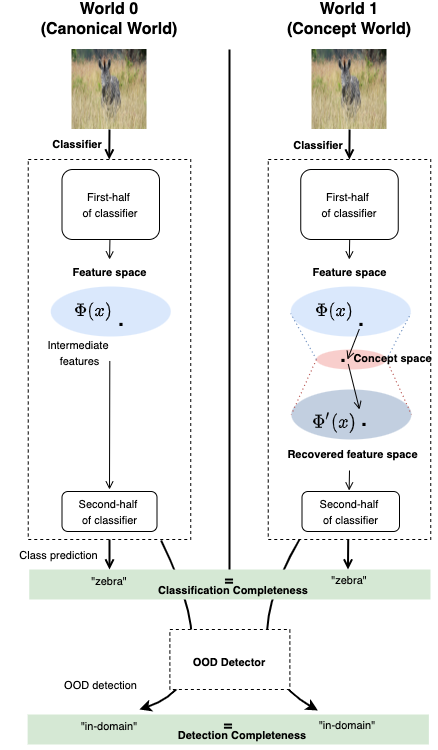
\includegraphics[width=0.45\textwidth]{figures/completeness.png}
% 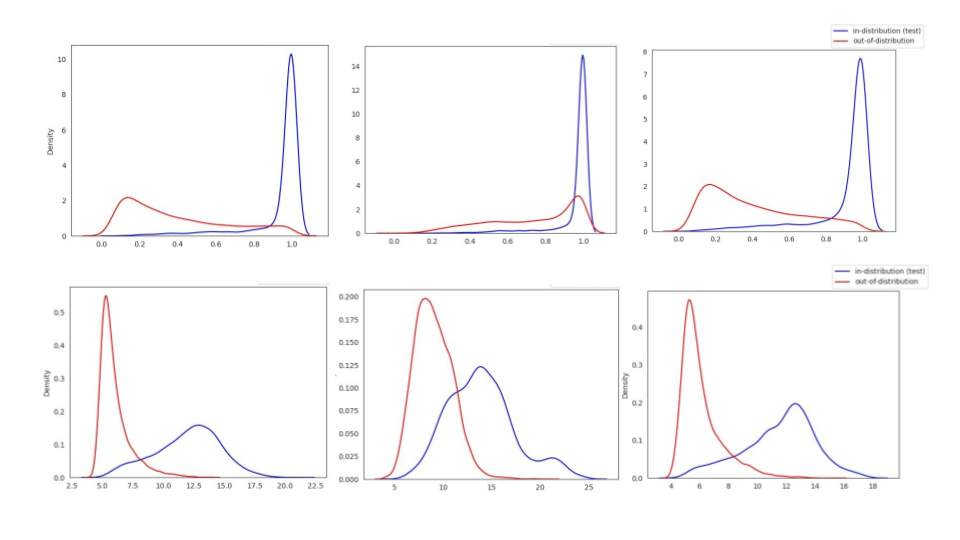
\includegraphics[scale=0.24]{figures/distribution.png}
% %\vspace{-2mm}
% \caption{Blue line is the estimated density of outputs from $\calD$ given ID test data (AwA), and red line is that of OOD test data (SUN). DNN classifier is Inception-V3 trained with AwA dataset.
% \textbf{First row}: distributions of outputs from MSP detector \citep{hendrycks2016msp}. 
% \textbf{Second row}: distributions of outputs from Energy detector \citep{liu2020energy}.
% \textbf{Left}: Target distribution of $S(\bfx, \bff)$ in canonical world. 
% \textbf{Mid}: Distribution of $S(\bfx, \fcon)$ in concept world, using concepts learned by \citep{yeh2020completeness}.
% \textbf{Right}: Distribution of $S(\bfx, \fcon)$ in concept world, using concepts learned by our framework.}
% \vspace{-5mm}
% \label{fig:score-distribution}
% \end{figure}
%

% \mypara{Limitations of Prior Work for OOD detectors.} 
While the objective (\ref{equ: baseline}) of \citeauthor{yeh2020completeness} can learn a set of sufficient concepts that have a high classification completeness score, we find that it does not necessarily replicate the per-instance prediction behavior of the classifier in the concept world. 
Specifically, there can be discrepancies in the reconstructed feature representation, whose effect propagates through the remaining part of the classifier. %to the output of the classifier.
% For instance, the empirical distribution of the prediction logits (pre-softmax layer) for both ID and OOD data based on the reconstructed feature representations could be very different from that based on the original feature representations.
Since many widely-used OOD detectors rely on the feature representations and/or the classifier's predictions, this discrepancy in the existing concept learning approaches makes it hard to closely replicate the OOD detector in the concept world (see Fig.~\ref{fig:score-distribution-msp}).
%
Furthermore, the scope of \citeauthor{yeh2020completeness} is confined to concept learning for explaining the classifier's predictions based on ID data, and there is no guarantee that the learned concepts would be useful for explaining an OOD detector. 
% In fact, the distribution of concept scores from ID and OOD data could be quite different (see Fig.~\ref{fig:score-distribution}).
% We illustrate this effect with a concrete example in Section~\ref{subsec:results}, when comparing the concept-score distributions from ID and OOD data based on the method of \citet{yeh2020completeness} and the proposed method.
%
To address these gaps, we propose a general method for concept learning that complements prior work by imposing additional instance-level constraints on the concepts, and by considering both the OOD detector and OOD data.
%
% We propose a general method for concept learning that overcomes the above gaps. Our method complements prior work by imposing additional instance-level constraints on the concepts, and by considering both the OOD detector and OOD data, as explained below.

\iffalse

% Earlier version
Unfortunately, there is a caveat with their approach.
Eqn. (\ref{equ: baseline}) may encourage the concepts to have high classification completeness score (defined in Eqn. (\ref{equ: completeness-classification})), but their concepts may fail to reduce the gap between canonical world and concept world genuinely. \ryan{By ensuring that they achieve an}
\textit{accurate reconstruction} of $\hat{\calZ}$
, the resulted concept scores would be sufficient enough to recover the accuracy of $\bff$ in expectation, but it is unclear whether the per-instance behavior of $\bff$ (and moreover, $\calD$ that runs based on $\bff$) is genuinely imitated.
To be more specific, $\bfC$ would be a set of $m$ principal vectors 
the set of concept vectors
$m$ unit vectors that fully span the space supported by $\{\bfphi(\bfx_1), \cdots, \bfphi(\bfx_{\Nintr})$.
usually not independent to each other (\eg concept "Greenery" is negatively related to concept "Sea").
have no guarantee on how \textit{accurate} the concepts are in explaining the classifier and the OOD detector.
% The reason we should care about in instance-level behavior of $\bff$ and $\calD$ in concept world is as follows. 
Besides, since the focus of \citep{yeh2020completeness} is initially confined to studying the utility of concepts for classifier with ID data, there is no guarantee for the utility of concepts for OOD detector explanations and in fact they distributions in concept space could be quite different for both ID and OOD data. We illustrate this effect with a concrete example in Section~\ref{subsec:results} when comparing the score distributions between ID and OOD on Yeh et al.~\citep{yeh2020completeness} and our approach to evaluate our reconstructed feature space $\hat{\calZ}$. To this end, we propose a general framework for concept learning that complements the previous works by additionally imposing instance-level requirements for concepts, and taking OOD data and OOD detector into consideration.

\fi

% \begin{equation}
% \label{equ: baseline+l2}
%     \argmax_{\bfC, g} \, \text{log} \proba_{(\bfx, y) \sim D^{train}_{in}}[\, h_{y}(\hat{\phi}_{g, \bfC}(\bfx))] + \lambda_1 \cdot R_{coherency}(\bfC) + \lambda_2 \cdot
%     \expec_{\bfx \sim D_{train}^{in}}||\phi(\bfx) - \hat{\phi}_{g, \bfC}(\bfx))||_2
% \end{equation}
% \begin{equation}
% \label{equ: baseline+score}
%     \argmax_{\bfC, g} \, \log \proba_{(\bfx, y) \sim D^{train}_{in}}[\, h_{y}(\hat{\phi}_{g, \bfC}(\bfx))] ~+~ \lambda\, R_{coherency}(\bfC) ~-~ \alpha \expec_{\bfx \sim D_{train}^{in}} (\mathcal{D}(h(\hat{\phi}_{g, \bfC}(\bfx))) - \mathcal{D}(f(\bfx)))^2
% \end{equation}

% Let $D^{train} = \{D_{\text{in}}^{train} \cup D_{\text{out}}^{train}\}$, and data is drawn as $(\bfx, s) \sim D^{train}$ where $s \in \{0, 1\}$ is the groundtruth label of OOD detection.
%
% \begin{equation}
% \label{equ: baseline+separability}
%     \argmax_{\bfC, g} \, \log \proba_{(\bfx, y) \sim D^{train}_{in}}[\, h_{y}(\hat{\phi}_{g, \bfC}(\bfx))] ~+~ \lambda\, R_{coherency}(\bfC) ~+~ \beta \expec_{\bfx \sim D^{train}} J(\bfC)
% \end{equation}
%

% \ap{Footenotetext for the algorithm is not appearing on the correct page. We may need to move it up or down when we get closer to the final draft.}

\mypara{Concept Learning Objective.}
We define a concept learning objective that aims to find a set of concepts $\bfC$ and a mapping $\bfg$ that have the following properties: 1) high detection completeness w.r.t the OOD detector; 2) high classification completeness w.r.t the DNN classifier; and 3) high separability in the concept-score space between detected-ID data and detected-OOD data.

\begin{figure*}[t]
  \centering
  \begin{subfigure}{0.32\linewidth}
    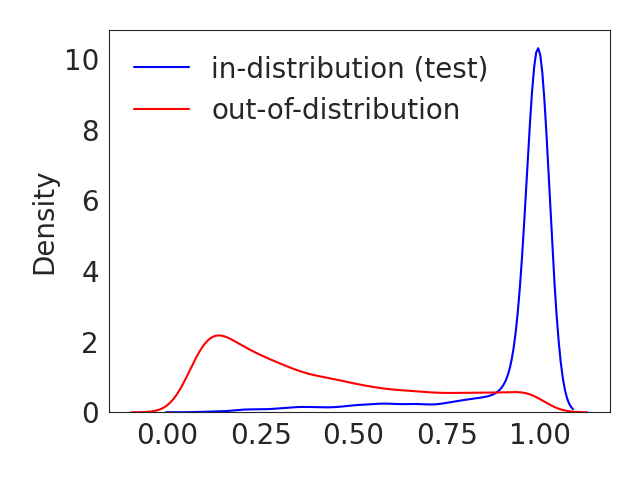
\includegraphics[width=\textwidth]{figures/distr_msp_target.png}
    \caption{\small Empirical distribution of $S(\bfx, \bff)$ from the target detector.}
    \label{fig:short-a}
  \end{subfigure}
  \hfill
  \begin{subfigure}{0.32\linewidth}
    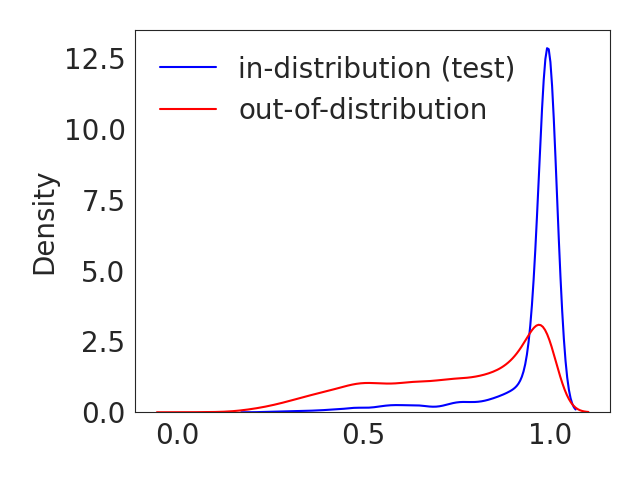
\includegraphics[width=\textwidth]{figures/distr_msp_yeh.png}
    \caption{\small Distribution of $\Scon(\bfx, \bff)$ using the concepts learned by \citet{yeh2020completeness}.}
    \label{fig:short-b}
  \end{subfigure}
  \hfill
  \begin{subfigure}{0.32\linewidth}
    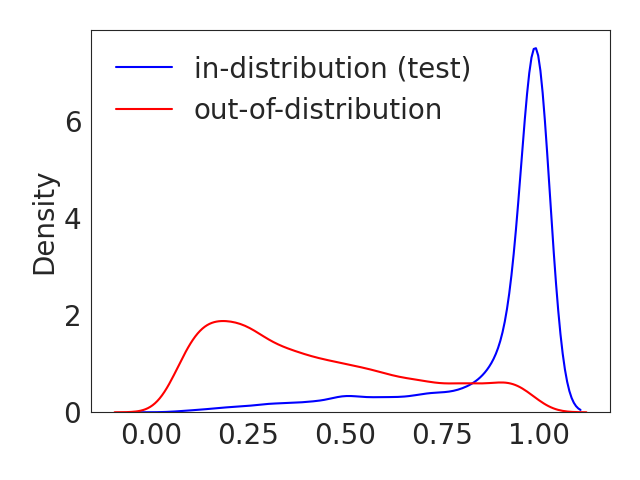
\includegraphics[width=\textwidth]{figures/distr_msp_ours.png}
    \caption{\small Distribution of $\Scon(\bfx, \bff)$ using the concepts learned by our method.}
    \label{fig:short-c}
  \end{subfigure}
  \caption{\small Empirical distribution of: \textbf{(a)} MSP detector score $S(\bfx, \bff)$ in the canonical world vs. \textbf{(b, c)} Reconstructed $\Scon(\bfx, \bff)$ in the concept world using the concepts learned by \citet{yeh2020completeness} and our method.
  Concepts learned by~\citet{yeh2020completeness} have $\eta^{}_{\bff} = 0.977, ~\eta^{}_{\bff, S}(\bfC) = 0.782$, while the concepts learned by our method $(\lambda_\textrm{mse} = 10, \lambda_\textrm{norm} = 0.1, \lambda_\textrm{sep} = 50)$ have $\eta^{}_{\bff} = 0.984, ~\eta^{}_{\bff, S}(\bfC) = 0.961$. 
  The AwA test set and the \texttt{SUN} dataset are used as ID (blue) and OOD (red) respectively.
    % Comparison is made between AwA test set (ID; blue) vs. \texttt{SUN} (OOD; red).
    }
    \vspace{-.1in}
\label{fig:score-distribution-msp}
\end{figure*}

% between the samples detected as ID and the samples detected as OOD by the detector. 
Inspired by recent works on transferring feature information from a teacher model to a student model~\citep{hinton2015distilling,zhou2018rocket},
% Recall that $\bfC$ projects from the original feature-representation space $\calZ$ to the concept-score space, which is then mapped to the reconstructed feature-representation space $\hat{\calZ}$ by $\bfg$.
we encourage accurate reconstruction of $\hat{\calZ}$ based on the concept scores by adding a regularization term that is the squared $\ell_2$ distance between the original and reconstructed representations $\,J_{\textrm{norm}}(\bfC, \bfg) ~=~ \expec_{\bfx \sim \Pin} \|\bfphi(\bfx) \,-\, \recphi(\bfx)\|^2\,$.
%
% \begin{align}
% \label{equ:regularizer_norm}
%     J_{\textrm{norm}}(\bfC, \bfg) ~=~ \expec_{\bfx \sim \Pin} \|\bfphi(\bfx) \,-\, \recphi(\bfx)\|^2.
% \end{align}
%
In order to close the gap between the scores of the OOD detector in the concept world and canonical world on a per-sample level, we introduce the following mean-squared-error (MSE) based regularization:
\begin{align}
\label{equ:regularizer_mse}
    J_{\textrm{mse}}(\bfC, \bfg) ~&=~ \expec_{\bfx \sim \Pin} \big( S(\bfx, \bfh \circ \recphi) - S(\bfx, \bff) \big)^2 \nonumber \\
    &~+~ \expec_{\bfx \sim \Pout} \big( S(\bfx, \bfh \circ \recphi) - S(\bfx, \bff) \big)^2 .
\end{align}
MSE terms are computed with both the ID and OOD data because we want to ensure that the ROC curve corresponding to both the score functions are close to each other (which requires OOD data).
Finally, we include a regularization term to maximize the separability metric between the detected-ID and detected-OOD data in the concept-score space, resulting in our final concept learning objective:
% We use the separability metric discussed in Section~\ref{sec:separability_score} directly as the regularization term since it is differentiable and tractable to optimize via gradient updates.
% With all regularization terms considered, 
%\vspace{-3mm}
\begin{align}
\label{equ: concept learning}
&\argmax_{\bfC, \bfg}  \expec_{(\bfx, y) \sim \Pin}\!\!\big[ \log h_y(\bfg(\VC(\bfx))) \big] ~+~ \lambda_{\textrm{expl}}\, R_{\textrm{expl}}(\bfC) \nonumber \\ 
    &-~ \lambda_{\textrm{mse}}\, J_{\textrm{mse}}(\bfC, \bfg) ~-~ \lambda_{\textrm{norm}}\, J_{\textrm{norm}}(\bfC, \bfg) ~+~ \lambda_{\textrm{sep}}~J_{\textrm{sep}}(\bfC).
\end{align}
The $\lambda$ coefficients are non-negative hyper-parameters that are further discussed in Section~\ref{subsec:results}.
We note that both $J_{\textrm{mse}}(\bfC, \bfg)$ and $J_{\textrm{sep}}(\bfC)$ depend on the OOD detector~\footnote{This dependence may not be obvious for the separability term, but it is clear from its definition.}.
% In case of the latter, this is clear from its definition, but may not obvious.
% The sign on the $\ell_2$ norm-based regularization and the MSE regularization terms is negative since we aim to minimize them.
% We use stochastic gradient descent-based optimization with adaptive learning rate (specifically Adam~\citep{kingma2014adam}) to solve the learning objective.
We use the SGD-based Adam optimizer~\citep{kingma2014adam}) to solve the learning objective.
The expectations involved in the objective terms are calculated using sample estimates from the training ID and OOD datasets. 
Specifically, $\Dintr$ and $\Douttr$ are used to compute the expectations over $\Pin$ and $\Pout$, respectively.
% The expectations involved in each of the terms in the objective are calculated using sample estimates from the training ID and OOD datasets. 
% Specifically, $\Dintr$ is used to compute the expectation over $\Pin$, and $\Douttr$ is used to compute the expectation over $\Pout$.
Our complete concept learning is summarized in Algorithm \ref{alg:concept_learning} (Appendix \ref{sec:appendix-algo}).



\iffalse

Detailed discussion of concept scores:

\mypara{Concept Scores.}
We start by formalizing how to compute a representative score for concepts given an input, which will be used for evaluation in Section \ref{sec:completeness_score} and Section \ref{sec:separability_score}.
We refer the reader to Section~\ref{sec:concept_projection}, which introduced a projection matrix $\bfC \in \reals^{d_\ell \times m}$ that maps $\bfphi(\bfx)$ to $\bfv_{\bfC}(\bfx)$ and consists of $m$ unit (column) concept vectors $\,\bfC := [\bfc_1 \cdots \bfc_m]$. 
The inner product between the feature representation and a concept vector quantifies how close the input is to the given concept, and this is referred to as the {\em concept score}. \ap{Does this need a cite? or is this our term?}
Specifically, the concept score corresponding to concept $i$ is $\bfv_{\bfc_i}(\bfx) = \langle \bfphi(\bfx), \bfc_i \rangle \in \reals^{a_\ell b_\ell}$, which is the $a_\ell \times b_\ell$ times concatenation over the standard inner-products (between vectors) $\,\langle \bfphi^{p,q}(\bfx), \bfc_i \rangle \in \reals, ~\forall p, q \in [a_\ell] \times [b_\ell]$, where $\bfphi^{p,q}$ is the feature representation corresponding to the $(p, q)$-th patch of input $\bfx$ (\ie receptive field).
That is, $\bfv_{\bfc_i}^{(p,q)}(\bfx)$ is the concept score of $(p, q)$-th patch of $\bfx$ with respect to $i$-th concept, and if it is a large positive (or negative) value, then the corresponding part of input is positively (or negatively) aligned with the concept.
The vector of concept scores from all the concepts is defined simply as the concatenation of the individual concept scores, \ie $\VC(\bfx)^T = [\bfv_{\bfc_1}(\bfx)^T, \cdots, \bfv_{\bfc_m}(\bfx)^T] \in \reals^{a_\ell b_\ell m}$.

% When $p = q = 1$ for fully-connected layers (\ie the receptive field of $\bfphi$ corresponds to the entire input $\bfx_i$), $\langle \bfphi(\bfx_i),~\bfc_j \rangle$ is a scalar concept score that represents the input.
% On the other hand, when $p, q > 1$, to obtain a scalar concept score for a given input, we take the maximum absolute concept score across the $p \times q$ patches, corresponding to $p \times q$ feature representations.
% To define the overall closeness of an input $\bfx_i$ and the concept $\bfc_j$ with a scalar concept score, we take the maximum absolute concept score across the $p \times q$ patches of $\bfx_i$.

\ap{Are p and q referring to the patch position? If so, why are (1,1), (1, -), and (-, 1) excluded by p, q > 1?}

When $p, q > 1$ (unless a fully-connected layer is of interest), where the receptive field of $\bfphi$ corresponds to the entire input $\bfx_i$), we also define a dimension-reduced version of the concept score vector that takes the maximum of the inner-product over each $a_\ell \times b_\ell$ patch (instead of concatenating them) as follows: $\TVC(\bfx)^T = [\widetilde{v}_{\bfc_1}(\bfx), \cdots, \widetilde{v}_{\bfc_m}(\bfx)] \in \reals^m$, where $\widetilde{v}_{\bfc_i}(\bfx) = \max_{p, q} |\langle \bfphi^{p,q}(\bfx), \bfc_i \rangle| \in \reals$.
% The intuition behind taking a maximum score across the patches of input is as follows.
This reduction operation is done to capture the most important correlations from each patch.
Suppose $\bfc_j$ represents a striped pattern and $\bfx_i$ is an image of a zebra standing on grass.
The patch of greenery background should get a low concept score, while a patch of the zebra's body should get high concept score.
% As the defining score for the stripe concept, we decide to take the score from the patch of zebra's body, out of all patches constituting the entire input image.
Out of all the patches constituting the input image, we take the maximum score (likely) corresponding to a patch of the zebra's body as the defining score for the striped concept.

Based on the concept scores and data defined as above, we elaborate the evaluation criteria of concepts for the purpose of OOD detector explanation in Section \ref{sec:completeness_score} and Section \ref{sec:separability_score}, followed by a general learning algorithm to discover concepts that satisfy the criteria in Section \ref{sec:concept_learning}.


\fi


% \begin{figure}[tbp]
% \centering
% \subfloat[MSP, target \label{fig:distr_msp_target}]{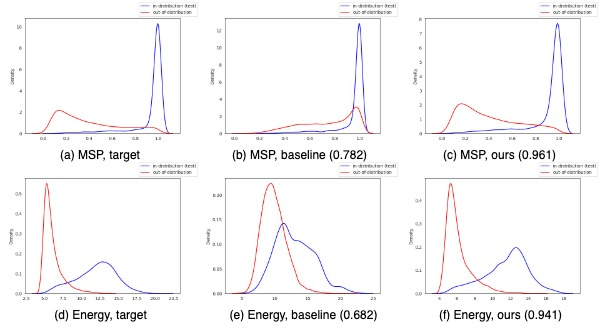
\includegraphics[width=0.3\textwidth]{figures/score_distribution.jpg}}\hfill
% \subfloat[Energy, ours\label{fig:distr_energy_ours}]{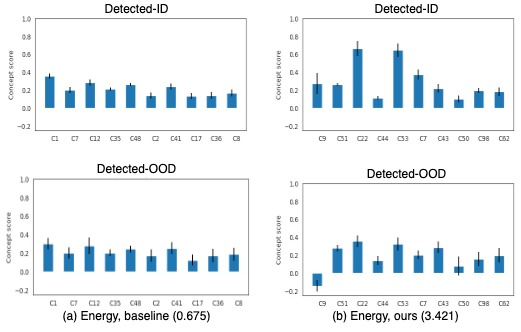
\includegraphics[width=0.3\textwidth]{figures/visual_dstinct.jpg}}
% \caption{
% \small \textbf{Estimated density of the score $S(\bfx, \bff)$ from Energy detector ~\citep{liu2020energy}}. 
% ID data is AwA test set (blue) and OOD data is the SUN dataset ~\citep{xiao2010sun} (red).
% \textbf{Left}: Target distribution of $S(\bfx, \bff)$ in the canonical world. 
% \textbf{Mid}: Distribution of $\Scon(\bfx, \bff)$ in the concept world, using concepts learned by \citep{yeh2020completeness} ($\,\lambda_\textrm{mse} = \lambda_\textrm{norm} = \lambda_\textrm{sep} = 0$).
% \textbf{Right}: Distribution of $\Scon(\bfx, \bff)$ in the concept world, using concepts learned by our method ($\,\lambda_\textrm{mse} = 1, \lambda_\textrm{norm} = 0.1, \lambda_\textrm{sep} = 50$ for Energy).
% % For MSP we set $\lambda_\textrm{mse} = 10, \lambda_\textrm{norm} = 0.1, \lambda_\textrm{sep} = 0$, and 
% }
% \label{fig:score-distribution}
% %\vspace{-5mm}
% \end{figure}

